\documentclass[]{article}
\usepackage{parskip}
\usepackage{pslatex}
\usepackage{graphicx}
\setlength{\parindent}{0.5cm}
\setlength{\parskip}{0pt}

\usepackage{tikz}

\usepackage{stmaryrd}

\usepackage{amsmath}
\usepackage{amsfonts}
\usepackage{amssymb}


\begin{document}

Johannes Kasimir

\section*{Task 1: Q-N with Anderson Acceleration}

Definitions:
\begin{equation}
    \mathbf{x}^{k+1} := \mathbf{N}(\mathbf{D}(\mathbf{x}^k))
\end{equation}
is the DN iteration on the interface Dirichlet values $\mathbf{x}^k := \{\mathbf{u}_\Gamma^{L,k}, \mathbf{u}_\Gamma^{R,k} \}$ where $L$ and $R$ signifies the left respectively the right shared interface in the room geometry.
\begin{align}
    \mathbf{H}(\mathbf{x}) = \mathbf{N}(\mathbf{D}(\mathbf{x}))
\end{align}
is the relaxed DN iteration and
\begin{equation}
    \mathbf{R}(\mathbf{x}) = \mathbf{H}(\mathbf{x}) - \mathbf{x}
\end{equation}
is the residual.

Using a Quasi-Newton method we want to solve the problem $\mathbf{R}(\mathbf{x})=0$.
Define the matrices
\begin{align}
    &\mathbf{V}_k = \begin{bmatrix}
        \mathbf{R}(\mathbf{x}^1) - \mathbf{R}(\mathbf{x}^0), &
         \ldots, &
         \mathbf{R}(\mathbf{x}^k) - \mathbf{R}(\mathbf{x}^{k-1})
    \end{bmatrix} \\
    &\mathbf{W}_k = \begin{bmatrix}
    \mathbf{x}^1 - \mathbf{x}^0, &
    \ldots, &
    \mathbf{x}^k - \mathbf{x}^{k-1}
    \end{bmatrix}.
\end{align}
The "Newton-updates" are defined by
\begin{equation}
    \Delta\mathbf{x}^k := \mathbf{W}_k \alpha
\end{equation}
where
\begin{equation}
    \alpha := argmin_\alpha || \mathbf{V}_k \alpha - \mathbf{R}(\mathbf{x}^k) ||_2.
\end{equation}
and the next interface Dirichlet values are
\begin{equation}
    \mathbf{x}^{k+1} = \mathbf{x}^k + \Delta \mathbf{x}^k.
\end{equation}


My first impression of this method was that it is significantly more robust than using optimal relaxation parameters. Changing the time step size or heat conductivity and -capacity barely influences the number of iterations required to convergence. However, the mesh width does influence the convergence rate, reducing $\Delta x$ increases the number of iterations required. We did not investigate the relationship between the convergence rate and $\Delta x$ closer, but the number of iterations required appears to be approximately inversely proportional to $\Delta x$. The high number of iterations required might indicate a bug in the code.

From the convergence history in figure \ref{qn} we see that most of the convergence happens in the last few iterations, a behavior resembling GMRES. But in contrast to GMRES the residual increases in some iterations. This can be compared to the DN iteration in figure \ref{dn} which has the expected log-linear convergence history of a linear iterative method. The DN iteration using optimal smoothing parameters converges faster, but finding the optimal smoothing parameter can be difficult. When $\Delta t$ grows large the optimal smoothing parameter approaches the expected limit value $\lambda_N/(\lambda_{D} + \lambda_N)$ but for smaller/intermediate size $\Delta t$ the value might be far from either of the limits $c\to 0$ or $c\to \inf$.

When $\lambda=\alpha=1$ then the solution reaches the steady state of the heat equation in relatively few time steps. When this happens the convergence rates of the DN and QN iterations increase until they always converge in a single step. This is natural since in the stationary state nothing changes in-between time steps, and therefore our initial guess for the interface Dirichlet values is already at the fixed point of the iterations.


\begin{figure}
	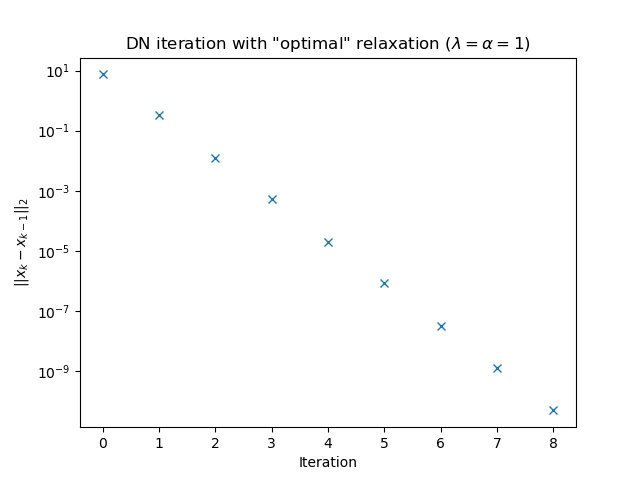
\includegraphics[width=0.9\linewidth]{dn_1.png}
	\caption{\label{dn} Convergence history for the DN iteration in the first time step. The relaxation parameter was not optimized exactly but by trial and error, $\theta=0.64$.}
\end{figure}

\begin{figure}
	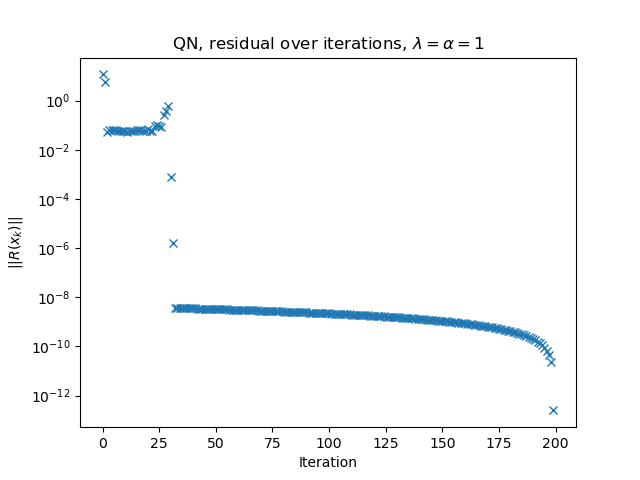
\includegraphics[width=0.9\linewidth]{qn_1.png}
	\caption{\label{qn} Convergence history for the QN iteration in the first time step.}
\end{figure}

\begin{figure}
	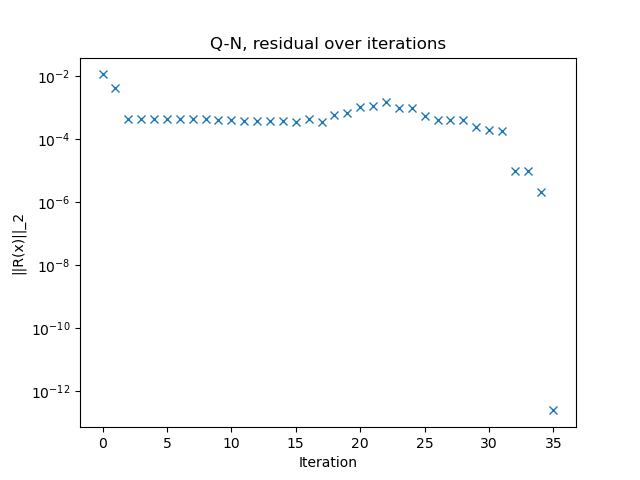
\includegraphics[width=0.9\linewidth]{qn.png}
	\caption{\label{qn} Convergence history for the QN iteration in a typical time step when $\lambda=0.0234$ and $\alpha=1300$.}
\end{figure}

\begin{figure}
	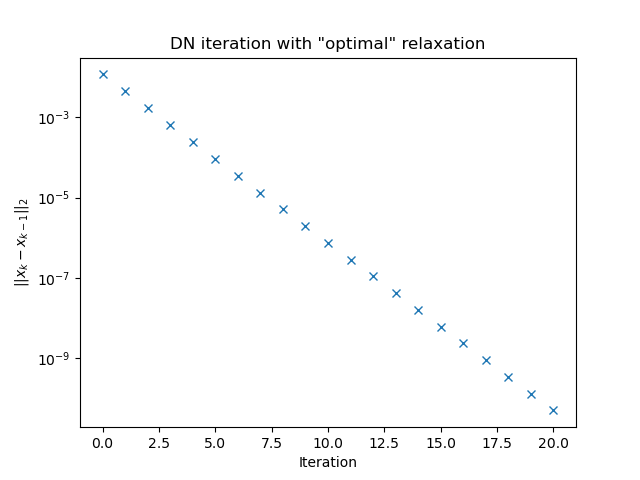
\includegraphics[width=0.9\linewidth]{dirichlet_neumann.png}
	\caption{\label{dn} Convergence history for the DN iteration in a typical time step when $\lambda=0.0234$ and $\alpha=1300$. The relaxation parameter was not optimized exactly but by trial and error, $\theta=0.62$.}
\end{figure}

\newpage

\section{Task 2: SDIRK for scalar ODE}

We are solving the equation:
\begin{equation}
\frac{d}{dt}\mathbf{u}(t) = \mathcal{L}(t, \mathbf{u}(t))
\end{equation}
where $\mathcal{L}$ is a possibly nonlinear operator acting on $u(t)$.
The time integration is done using an adaptive SDIRK, \textit{diagonally implicit Runge Kutta} method, of the form
\begin{align}
\mathbf{u}_{n+1} &= \mathbf{u}_n + h \sum_{i=1}^{s} b_i\mathbf{k}_i \\
\mathbf{k}_i &= \mathcal{L}(t_n + c_i h, \mathbf{u}_n + h\sum_{j=1}^{i} a_{ij} \mathbf{k}_j).
\end{align}
A DIRK scheme is executed by solving a series of nonlinear equation systems. At each stage $i$, solve
\begin{align}
\label{eq:stage}
\mathbf{k}_i &= \mathcal{L}(\bar{t}_i, \bar{´\mathbf{u}}_i + \alpha_i \mathbf{k}_i)
\end{align}
where $\alpha_i = h a_{ii}$ and $\bar{t}_i$ is a prescribed time, $\bar{\mathbf{u}}_i$ is a linear combination of the steps from previous stages and the point $\mathbf{u}_n$.

In our case the operator is
\begin{equation}
    \mathcal{L}(t, \mathbf{u}) = \begin{bmatrix} 0 & 1 \\ -k/m & 0\end{bmatrix}\mathbf{u} + \frac{A}{m} \begin{bmatrix} 0 \\ p(t)-p_0\end{bmatrix}
\end{equation}
and the system we need to solve every stage is
\begin{equation}
(\mathbf{I} - \alpha_i \begin{bmatrix} 0 & 1 \\ -k/m & 0\end{bmatrix})\mathbf{k}_i  = \begin{bmatrix} 0 & 1 \\ -k/m & 0\end{bmatrix}\bar{\mathbf{u}}_i + \frac{A}{m} \begin{bmatrix} 0 \\ p(t)-p_0\end{bmatrix}.
\end{equation}

The method should be time adaptive. This is achieved using an embedded RK method of order $\hat{p} < p$ where $p$ is the order of the SDIRK method. At the end of every timestep, the error is estimated by
\begin{equation}
    \hat{\mathbf{e}} = \sum_{i=1}^s d_i \mathbf{k}_i
\end{equation}
for some constants $d_i$ given by the method. The next time step is calculated as
\begin{equation}
    \Delta t := 0.9 \Delta t \bigg(\frac{TOL}{||\hat{\mathbf{e}}||}\bigg)^{\frac{1}{\hat{p}+1}}.
\end{equation} 

\begin{figure}
	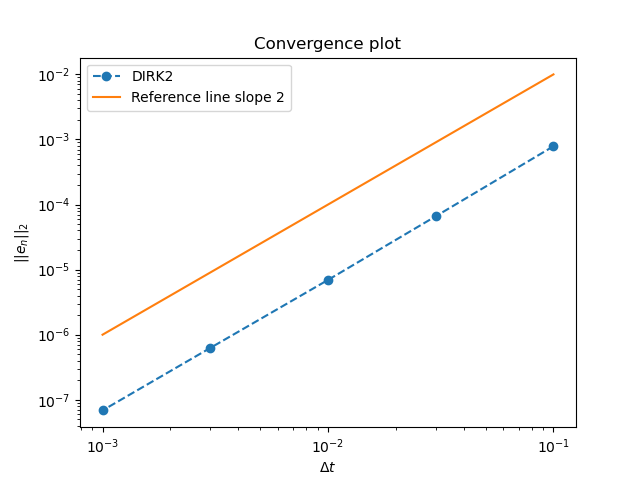
\includegraphics[width=0.9\linewidth]{error.png}
	\caption{\label{sdirk2} Error at last time step over $\Delta t$.}
\end{figure}	
\begin{figure}
	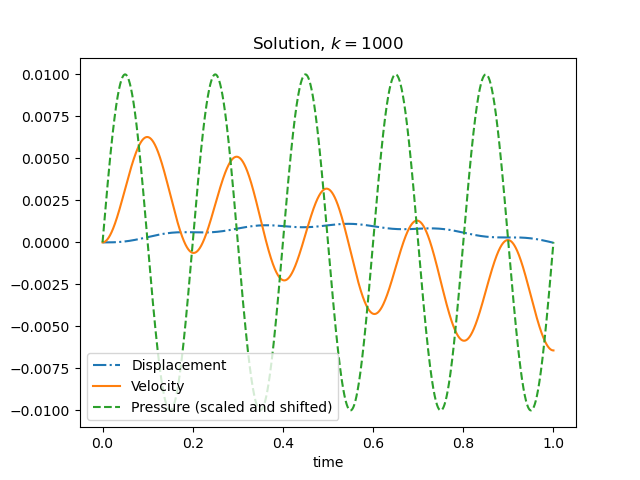
\includegraphics[width=0.9\linewidth]{solution.png}
	\caption{\label{solution}
	}
\end{figure}	
\begin{figure}
	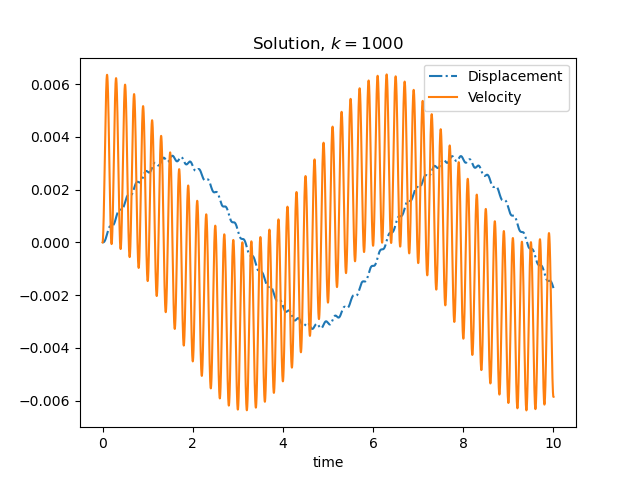
\includegraphics[width=0.9\linewidth]{solutionk100.png}
	\caption{\label{solutionk100} Lower stiffness leads to larger deformations and a lower characteristic frequency of the piston.}
\end{figure}

\end{document}
